%% bare_conf.tex
%% V1.4
%% 2012/12/27
%% by Michael Shell
%% See:
%% http://www.michaelshell.org/
%% for current contact information.
%%
%% This is a skeleton file demonstrating the use of IEEEtran.cls
%% (requires IEEEtran.cls version 1.8 or later) with an IEEE conference paper.
%%
%% Support sites:
%% http://www.michaelshell.org/tex/ieeetran/
%% http://www.ctan.org/tex-archive/macros/latex/contrib/IEEEtran/
%% and
%% http://www.ieee.org/

%%*************************************************************************
%% Legal Notice:
%% This code is offered as-is without any warranty either expressed or
%% implied; without even the implied warranty of MERCHANTABILITY or
%% FITNESS FOR A PARTICULAR PURPOSE! 
%% User assumes all risk.
%% In no event shall IEEE or any contributor to this code be liable for
%% any damages or losses, including, but not limited to, incidental,
%% consequential, or any other damages, resulting from the use or misuse
%% of any information contained here.
%%
%% All comments are the opinions of their respective authors and are not
%% necessarily endorsed by the IEEE.
%%
%% This work is distributed under the LaTeX Project Public License (LPPL)
%% ( http://www.latex-project.org/ ) version 1.3, and may be freely used,
%% distributed and modified. A copy of the LPPL, version 1.3, is included
%% in the base LaTeX documentation of all distributions of LaTeX released
%% 2003/12/01 or later.
%% Retain all contribution notices and credits.
%% ** Modified files should be clearly indicated as such, including  **
%% ** renaming them and changing author support contact information. **
%%
%% File list of work: IEEEtran.cls, IEEEtran_HOWTO.pdf, bare_adv.tex,
%%                    bare_conf.tex, bare_jrnl.tex, bare_jrnl_compsoc.tex,
%%                    bare_jrnl_transmag.tex
%%*************************************************************************

% *** Authors should verify (and, if needed, correct) their LaTeX system  ***
% *** with the testflow diagnostic prior to trusting their LaTeX platform ***
% *** with production work. IEEE's font choices can trigger bugs that do  ***
% *** not appear when using other class files.                            ***
% The testflow support page is at:
% http://www.michaelshell.org/tex/testflow/



% Note that the a4paper option is mainly intended so that authors in
% countries using A4 can easily print to A4 and see how their papers will
% look in print - the typesetting of the document will not typically be
% affected with changes in paper size (but the bottom and side margins will).
% Use the testflow package mentioned above to verify correct handling of
% both paper sizes by the user's LaTeX system.
%
% Also note that the "draftcls" or "draftclsnofoot", not "draft", option
% should be used if it is desired that the figures are to be displayed inft.tex

% draft mode.
%\documentclass[a4paper, 10pt, conference]{ieeeconf}
\documentclass[letterpaper, 10pt, conference]{ieeeconf}
%\documentclass[12pt,a4paper,final]{article}
%\IEEEoverridecommandlockouts
%\overrideIEEEmargins
%\documentclass[conference]{IEEEtrans}
% Add the compsoc option for Computer Society conferences.
%
% If IEEEtran.cls has not been installed into the LaTeX system files,ft.tex

% manually specify the path to it like:
\usepackage{amssymb}
%\usepackage{amsthm}
%\usepackage{caption}
\usepackage{multirow}
\usepackage{setspace}
\usepackage{epstopdf}
%\usepackage{graphics} % for pdf, bitmapped graphics files
%\usepackage{epsfig} % for postscript graphics files
\usepackage{mathptmx} % assumes new font selection scheme installed
%\usepackage{times} % assumes new font selection scheme installed
%\usepackage{amsmath} % assumes amsmath package installed
\usepackage{amssymb}  % assumes amsmath package installed
\usepackage{fancyhdr}
% Some very useful LaTeX packages include:
% (uncomment the ones you want to load)


% *** MISC UTILITY PACKAGES ***
%
\usepackage{ifpdf}
% Heiko Oberdiek's ifpdf.sty is very useful if you need conditional
% compilation based on whether the output is pdf or dvi.
% usage:
% \ifpdf
%   % pdf code
% \else
%   % dvi code
% \fi
% The latest version of ifpdf.sty can be obtained from:
% http://www.ctan.org/tex-archive/macros/latex/contrib/oberdiek/
% Also, note that IEEEtran.cls V1.7 and later provides a builtin
% \ifCLASSINFOpdf conditional that works the same way.
% When switching from latex to pdflatex and vice-versa, the compiler may
% have to be run twice to clear warning/error messages.






% *** CITATION PACKAGES ***
%
\usepackage{cite}
% cite.sty was written by Donald Arseneau
% V1.6 and later of IEEEtran pre-defines the format of the cite.sty package
% \cite{} output to follow that of IEEE. Loading the cite package will
% result in citation numbers being automatically sorted and properly
% "compressed/ranged". e.g., [1], [9], [2], [7], [5], [6] without using
% cite.sty will become [1], [2], [5]--[7], [9] using cite.sty. cite.sty's
% \cite will automatically add leading space, if needed. Use cite.sty's
% noadjust option (cite.sty V3.8 and later) if you want to turn this off
% such as if a citation ever needs to be enclosed in parenthesis.
% cite.sty is already installed on most LaTeX systems. Be sure and use
% version 4.0 (2003-05-27) and later if using hyperref.sty. cite.sty does
% not currently provide for hyperlinked citations.
% The latest version can be obtained at:
% http://www.ctan.org/tex-archive/macros/latex/contrib/cite/
% The documentation is contained in the cite.sty file itself.






% *** GRAPHICS RELATED PACKAGES ***
%
%\ifCLASSINFOpdf
  % \usepackage[pdftex]{graphicx}
  % declare the path(s) where your graphic files are
  % \graphicspath{{../pdf/}{../jpeg/}}
  % and their extensions so you won't have to specify these with
  % every instance of \includegraphics
  % \DeclareGraphicsExtensions{.pdf,.jpeg,.png}
%\else
  % or other class option (dvipsone, dvipdf, if not using dvips). graphicx
  % will default to the driver specified in the system graphics.cfg if no
  % driver is specified.
  \usepackage[dvips]{graphicx}
  % declare the path(s) where your graphic files are
  % \graphicspath{{../eps/}}
  % and their extensions so you won't have to specify these with
  % every instance of \includegraphics
  % \DeclareGraphicsExtensions{.eps}
%\fi
% graphicx was written by David Carlisle and Sebastian Rahtz. It is
% required if you want graphics, photos, etc. graphicx.sty is already
% installed on most LaTeX systems. The latest version and documentation
% can be obtained at: 
% http://www.ctan.org/tex-archive/macros/latex/required/graphics/
% Another good source of documentation is "Using Imported Graphics in
% LaTeX2e" by Keith Reckdahl which can be found at:
% http://www.ctan.org/tex-archive/info/epslatex/
%
% latex, and pdflatex in dvi mode, support graphics in encapsulated
% postscript (.eps) format. pdflatex in pdf mode supports graphics
% in .pdf, .jpeg, .png and .mps (metapost) formats. Users should ensure
% that all non-photo figures use a vector format (.eps, .pdf, .mps) and
% not a bitmapped formats (.jpeg, .png). IEEE frowns on bitmapped formats
% which can result in "jaggedy"/blurry rendering of lines and letters as
% well as large increases in file sizes.
%
% You can find documentation about the pdfTeX application at:
% http://www.tug.org/applications/pdftex





% *** MATH PACKAGES ***
%
\usepackage[cmex10]{amsmath}
% A popular package from the American Mathematical Society that provides
% many useful and powerful commands for dealing with mathematics. If using
% it, be sure to load this package with the cmex10 option to ensure that
% only type 1 fonts will utilized at all point sizes. Without this option,
% it is possible that some math symbols, particularly those within
% footnotes, will be rendered in bitmap form which will result in a
% document that can not be IEEE Xplore compliant!
%
% Also, note that the amsmath package sets \interdisplaylinepenalty to 10000
% thus preventing page breaks from occurring within multiline equations. Use:
%\interdisplaylinepenalty=2500
% after loading amsmath to restore such page breaks as IEEEtran.cls normally
% does. amsmath.sty is already installed on most LaTeX systems. The latest
% version and documentation can be obtained at:
% http://www.ctan.org/tex-archive/macros/latex/required/amslatex/math/





% *** SPECIALIZED LIST PACKAGES ***
%
\usepackage{algorithmic}
% algorithmic.sty was written by Peter Williams and Rogerio Brito.
% This package provides an algorithmic environment fo describing algorithms.
% You can use the algorithmic environment in-text or within a figure
% environment to provide for a floating algorithm. Do NOT use the algorithm
% floating environment provided by algorithm.sty (by the same authors) or
% algorithm2e.sty (by Christophe Fiorio) as IEEE does not use dedicated
% algorithm float types and packages that provide these will not provide
% correct IEEE style captions. The latest version and documentation of
% algorithmic.sty can be obtained at:
% http://www.ctan.org/tex-archive/macros/latex/contrib/algorithms/
% There is also a support site at:
% http://algorithms.berlios.de/index.html
% Also of interest may be the (relatively newer and more customizable)
% algorithmicx.sty package by Szasz Janos:
% http://www.ctan.org/tex-archive/macros/latex/contrib/algorithmicx/




% *** ALIGNMENT PACKAGES ***
%
\usepackage{array}
% Frank Mittelbach's and David Carlisle's array.sty patches and improves
% the standard LaTeX2e array and tabular environments to provide better
% appearance and additional user controls. As the default LaTeX2e table
% generation code is lacking to the point of almost being broken with
% respect to the quality of the end results, all users are strongly
% advised to use an enhanced (at the very least that provided by array.sty)
% set of table tools. array.sty is already installed on most systems. The
% latest version and documentation can be obtained at:
% http://www.ctan.org/tex-archive/macros/latex/required/tools/


% IEEEtran contains the IEEEeqnarray family of commands that can be used to
% generate multiline equations as well as matrices, tables, etc., of high
% quality.




% *** SUBFIGURE PACKAGES ***
%\ifCLASSOPTIONcompsoc
%  \usepackage[caption=false,font=normalsize,labelfont=sf,textfont=sf]{subfig}
%\else
  \usepackage[caption=false,font=footnotesize]{subfig}
%\fi
% subfig.sty, written by Steven Douglas Cochran, is the modern replacement
% for subfigure.sty, the latter of which is no longer maintained and is
% incompatible with some LaTeX packages including fixltx2e. However,
% subfig.sty requires and automatically loads Axel Sommerfeldt's caption.sty
% which will override IEEEtran.cls' handling of captions and this will result
% in non-IEEE style figure/table captions. To prevent this problem, be sure
% and invoke subfig.sty's "caption=false" package option (available since
% subfig.sty version 1.3, 2005/06/28) as this is will preserve IEEEtran.cls
% handling of captions.
% Note that the Computer Society format requires a larger sans serif font
% than the serif footnote size font used in traditional IEEE formatting
% and thus the need to invoke different subfig.sty package options depending
% on whether compsoc mode has been enabled.
%
% The latest version and documentation of subfig.sty can be obtained at:
% http://www.ctan.org/tex-archive/macros/latex/contrib/subfig/




% *** FLOAT PACKAGES ***
%
%\usepackage{fixltx2e}
% fixltx2e, the successor to the earlier fix2col.sty, was written by
% Frank Mittelbach and David Carlisle. This package corrects a few problems
% in the LaTeX2e kernel, the most notable of which is that in current
% LaTeX2e releases, the ordering of single and double column floats is not
% guaranteed to be preserved. Thus, an unpatched LaTeX2e can allow a
% single column figure to be placed prior to an earlier double column
% figure. The latest version and documentation can be found at:
% http://www.ctan.org/tex-archive/macros/latex/base/


%\usepackage{stfloats}
% stfloats.sty was written by Sigitas Tolusis. This package gives LaTeX2e
% the ability to do double column floats at the bottom of the page as well
% as the top. (e.g., "\begin{figure*}[!b]" is not normally possible in
% LaTeX2e). It also provides a command:
%\fnbelowfloat
% to enable the placement of footnotes below bottom floats (the standard
% LaTeX2e kernel puts them above bottom floats). This is an invasive package
% which rewrites many portions of the LaTeX2e float routines. It may not work
% with other packages that modify the LaTeX2e float routines. The latest
% version and documentation can be obtained at:
% http://www.ctan.org/tex-archive/macros/latex/contrib/sttools/
% Do not use the stfloats baselinefloat ability as IEEE does not allow
% \baselineskip to stretch. Authors submitting work to the IEEE should note
% that IEEE rarely uses double column equations and that authors should try
% to avoid such use. Do not be tempted to use the cuted.sty or midfloat.sty
% packages (also by Sigitas Tolusis) as IEEE does not format its papers in
% such ways.
% Do not attempt to use stfloats with fixltx2e as they are incompatible.
% Instead, use Morten Hogholm'a dblfloatfix which combines the features
% of both fixltx2e and stfloats:
%
% \usepackage{dblfloatfix}
% The latest version can be found at:
% http://www.ctan.org/tex-archive/macros/latex/contrib/dblfloatfix/




% *** PDF, URL AND HYPERLINK PACKAGES ***
%
\usepackage{url}
% url.sty was written by Donald Arseneau. It provides better support for
% handling and breaking URLs. url.sty is already installed on most LaTeX
% systems. The latest version and documentation can be obtained at:
% http://www.ctan.org/tex-archive/macros/latex/contrib/url/
% Basically, \url{my_url_here}.




% *** Do not adjust lengths that control margins, column widths, etc. ***
% *** Do not use packages that alter fonts (such as pslatex).         ***
% There should be no need to do such things with IEEEtran.cls V1.6 and later.
% (Unless specifically asked to do so by the journal or conference you plan
% to submit to, of course. )


% correct bad hyphenation here
%\hyphenation{op-tical net-works semi-conduc-tor}



%
% paper title
% can use linebreaks \\ within to get better formatting as desired
% Do not put math or special symbols in the title.
\title{\LARGE \bf GPU Acceleration for Fixed Complexity Sphere Decoder in Large MIMO Uplink Systems}


% author names and affiliations
% use a multiple column layout for up to three different
% affiliations
%\author{\IEEEauthorblockN{Tianpei Chen} and 
%\IEEEauthorblockN{Harry Leib}}
%\IEEEauthorblockA{ID: 25504946\\Department of Electrical and\\Computer Engineering\\
%McGill University\\
%Montreal, Quebec}}
\author{Tianpei Chen and Harry Leib\\
Department of Electrical and Computer Engineering, McGill University, Montreal, Quebec\\
tianpei.chen@mail.mcgill.ca harry.leib@mcgill.ca}
 %Department of Electrical and Computer Engineering\\
 %McGill University\\
% Montreal, Quebec}

% conference papers do not typically use \thanks and this command
% is locked out in conference mode. If really needed, such as for
% the acknowledgment of grants, issue a \IEEEoverridecommandlockouts
% after \documentclass

% for over three affiliations, or if they all won't fit within the width
% of the page, use this alternative format:
% 
%\author{\IEEEauthorblockN{Michael Shell\IEEEauthorrefmark{1},
%Homer Simpson\IEEEauthorrefmark{2},
%James Kirk\IEEEauthorrefmark{3}, 
%Montgomery Scott\IEEEauthorrefmark{3} and
%Eldon Tyrell\IEEEauthorrefmark{4}}
%\IEEEauthorblockA{\IEEEauthorrefmark{1}School of Electrical and Computer Engineering\\
%Georgia Institute of Technology,
%Atlanta, Georgia 30332--0250\\ Email: see http://www.michaelshell.org/contact.html}
%\IEEEauthorblockA{\IEEEauthorrefmark{2}Twentieth Century Fox, Springfield, USA\\
%Email: homer@thesimpsons.com}
%\IEEEauthorblockA{\IEEEauthorrefmark{3}Starfleet Academy, San Francisco, California 96678-2391\\
%Telephone: (800) 555--1212, Fax: (888) 555--1212}
%\IEEEauthorblockA{\IEEEauthorrefmark{4}Tyrell Inc., 123 Replicant Street, Los Angeles, California 90210--4321}}


%\author{\IEEEauthorblockN{Tianpei Chen and
%Harry Leib
%}
%\IEEEauthorblockA{Department of Electrical and Computer Engineering\\
%McGill University, Montreal, Quebec, Canada}}




% use for special paper notices
%\IEEEspecialpapernotice{(Invited Paper)}



\begin{document}
% make the title area
%\begin{spacing}{2.5}
%\date{}
\maketitle
\thispagestyle{fancy} % IEEE模板在\maketitle后会自动声明\thispagestyle{plain},  
                      % 导致第一页什么都没有。所以得把plain更改为fancy  
\lhead{} % 页眉左,需要东西的话就在{}内添加  
\chead{} % 页眉中  
\rhead{\thepage} % 页眉右  
\lfoot{} % 页眉左  
\cfoot{} % 页眉中  
\rfoot{} %页眉右,\thepage 表示当前页码  
\renewcommand{\headrulewidth}{0pt} %改为0pt即可去掉页眉下面的横线  
\renewcommand{\footrulewidth}{0pt} %改为0pt即可去掉页脚上面的横线  
\pagestyle{fancy}  
\rhead{\thepage}
%\thispagestyle{empty}
%\pagestyle{empty}
% As a general rule, do not put math, special symbols or citations
% in the abstract
\begin{abstract}
Large MIMO constitutes a principal technology for next generation wireless communication systems. Detection algorithms for large MIMO schemes tend to require long simulation times on conventional computer systems. In order to improve simulation efficiency of decoders in large MIMO systems, we propose to use General Purpose Graphic Processing Units (GPGPU). This paper considers the implementation of a Fixed Complexity Sphere Decoder (FCSD) for large scale MIMO systems using the framework of GPGPU-Computed Unified Device Architecture (CUDA). The proposed CUDA-FCSD can achieve considerable speedups over conventional CPU implementation while providing the same Bit Error Rate (BER) performance. Furthermore the proposed algorithm demonstrates the great potential of GPGPU to accelerate the simulation of large MIMO systems.

\textbf{ Keywords: Large MIMO, fixed complexity sphere decoder (FCSD), general purpose graphic processing units (GPGPU), computed unified device architecture (CUDA)}
\end{abstract}

% no keywords




% For peer review papers, you can put extra information on the cover
% page as needed:
% \ifCLASSOPTIONpeerreview
% \begin{center} \bfseries EDICS Category: 3-BBND \end{center}
% \fi
%
% For peerreview papers, this IEEEtran command inserts a page break and
% creates the second title. It will be ignored for other modes.
%\IEEEpeerreviewmaketitle

\section{Introduction}
A present challenge in the wireless communication area is to bridge the sharp contrast between the increasing demand of mobile network speed for the transmission of rich media content with better QoS (Quality of Service), and the shortage of radio frequency spectrum. Multiple Input Multiple Output (MIMO) technology is of immense research interest since it can help solving this problem owing to several advantages it offers. The core idea of MIMO is to use multiple antennas at the transmitting and receiving sides, that provide parallel data pipes, resulting in spatial multiplexing and diversity gains\cite{oestges2010mimo}. 

Large scale MIMO (also named massive MIMO) systems employ tens to hundreds of low-power low-price antennas at the base station, that serve many terminals at the same time\cite{rusek2013scaling}. Large scale MIMO can achieve the full potential of conventional MIMO systems, as well as provide additional reduction of latency and improvement of system robustness. The detector is one of the key components of MIMO systems.
 A well known detector for MIMO systems is the Sphere Decoder (SD) that performs as well as a Maximum Likelihood detector (MLD), with a dramatic complexity reduction\cite{viterbo1999universal}\cite{hassibi2005sphere}. There are two major problems with the traditional SD decoder: complexity depending on Signal to Noise Ratio (SNR), and sequential nature, which conflict with the requirement of a constant data processing throughput and parallel implementation for practical systems. The Fixed Complexity Sphere Decoder (FCSD) overcomes these problems of the SD decoder by searching the solution along a fixed number of independent paths\cite{barbero2008fixing}.
 
General Purpose Graphic Processing Units (GPGPU) computing is a common trend in industry and research in areas that need massive computations, such as computer vision\cite{fung2008using}, computer games\cite{blewitt2013applicability}, signal processing\cite{van2011accelerating}\cite{6671435}, and finance\cite{grauer2013accelerating}. Compared to a CPU, a GPU can naturally cope with computational intensive tasks, since most of the hardware resources are allocated for data processing and parallel computation, rather than caching and flow control\cite{cook2013cuda}. In recent years GPU computing has provided significant advantages in data processing speeds over CPU computations\cite{nvidia2008programming}. The Computed unified Device Architecture (CUDA)\cite{cook2013cuda}\cite{nvidia2008programming} is a programming model for GPGPU that was proposed by NIVIDIA and has become the dominant framework for GPGPU programming. It is based on popular programming languages (C, C++, Java, Python, Fortran, Direct Compute), such that the application developers in different areas do not need to learn a new programming language or get to know the hardware details. CUDA employs the Single Instruction Multiple Threads (SIMT) programming model, enables a GPU to implement parallel data processing, and has become a parallel computing platform for different applications.

In this paper, a GPU based implementation of Fixed Complexity Sphere Decoder (FCSD) is proposed, which is referred to as CUDA-FCSD. A heterogeneous programming solution for FCSD preprocessing and integrated blocked parallel path searching and decision making are presented. Using this implementation the speedup as well as Bit Error Rate (BER) performance of different sizes of MIMO systems and signal constellations are analyzed. The proposed CUDA-FCSD implementation demonstrates a great potential for large MIMO systems.

The rest of the paper is organized as follows. Section \ref{programming model} briefly introduces CUDA, the GPU architecture and the programming model. In section \ref{GPUFCSD}, we present details of the implementation of CUDA-FCSD. In section \ref{simulation}, the speedup and bit error rate (BER) performance of CUDA-FCSD are considered. Finally, conclusions are drawn in section \ref{conclusion}.    
% An example of a floating figure using the graphicx package.
% Note that \label must occur AFTER (or within) \caption.

% For figures, \caption should occur after the \includegraphics.
% Note that IEEEtran v1.7 and later has special internal code that
% is designed to preserve the operation of \label within \caption
% even when the captionsoff option is in effect. However, because
% of issues like this, it may be the safest practice to put all your
% \label just after \caption rather than within \caption{}.
%
% Reminder: the "draftcls" or "draftclsnofoot", not "draft", class
% option should be used if it is desired that the figures are to be
% displayed while in draft mode.
%
%\begin{figure}[!t]
%\centering
%\includegraphics[width=2.5in]{myfigure}
% where an .eps filename suffix will be assumed under latex, 
% and a .pdf suffix will be assumed for pdflatex; or what has been declared
% via \DeclareGraphicsExtensions.
%\caption{Simulation Results.}
%\label{fig_sim}
%\end{figure}

% Note that IEEE typically puts floats only at the top, even when this
% results in a large percentage of a column being occupied by floats.


% An example of a double column floating figure using two subfigures.
% (The subfig.sty package must be loaded for this to work.)
% The subfigure \label commands are set within each subfloat command,
% and the \label for the overall figure must come after \caption.
% \hfil is used as a separator to get equal spacing.
% Watch out that the combined width of all the subfigures on a 
% line do not exceed the text width or a line break will occur.
%
%\begin{figure*}[!t]
%\centering
%\subfloat[Case I]{\includegraphics[width=2.5in]{box}%
%\label{fig_first_case}}
%\hfil
%\subfloat[Case II]{\includegraphics[width=2.5in]{box}%
%\label{fig_second_case}}
%\caption{Simulation results.}
%\label{fig_sim}
%\end{figure*}
%
% Note that often IEEE papers with subfigures do not employ subfigure
% captions (using the optional argument to \subfloat[]), but instead will
% reference/describe all of them (a), (b), etc., within the main caption.


% An example of a floating table. Note that, for IEEE style tables, the 
% \caption command should come BEFORE the table. Table text will default to
% \footnotesize as IEEE normally uses this smaller font for tables.
% The \label must come after \caption as always.
%
%\begin{table}[!t]
%% increase table row spacing, adjust to taste
%\renewcommand{\arraystretch}{1.3}
% if using array.sty, it might be a good idea to tweak the value of
% \extrarowheight as needed to properly center the text within the cells
%\caption{An Example of a Table}
%\label{table_example}
%\centering
%% Some packages, such as MDW tools, offer better commands for making tables
%% than the plain LaTeX2e tabular which is used here.
%\begin{tabular}{|c||c|}
%\hline
%One & Two\\
%\hline
%Three & Four\\
%\hline
%\end{tabular}
%\end{table}

\section{CUDA Programming Model and GPU Architecture} \label{programming model} 
\subsection{Single Instruction Multiple Thread Model}
The CUDA programming model is a C programming extension with special defined syntax and structure. The serial code is executed on the host (CPU) side, and massive parallel data processing is performed on the device (GPU) side. Such an approach is defined as a heterogeneous programming model. A thread is the basic programming unit of CUDA. A block of cooperative threads form a thread block, where they can synchronize their behavior and communicate. Fig. \ref{figure1} illustrates a simple CUDA memory hierachy model.
\begin{figure}[htb]
\centering
\includegraphics*[width=0.5\textwidth]{CUDA_programming_hierachy.eps}
\caption{ CUDA 3D memory hierachy $5\times 5\times 5$ grid, with each block composed of $5\times 5\times 5$ threads.
The threads can be organized into one-dimensional, two-dimensional or three-dimensional blocks. Similarly, blocks can also be grouped into a one-dimensional, two-dimensional, or three-dimensional grid.
}
\label{figure1}
\end{figure} 

Threads are scheduled, managed, created and executed in a group of 32, called warp. The programs that execute on the device side are defined as \textit{kernel} functions. When a \textit{kernel} function is invoked, the thread blocks are partitioned into warps. The threads in one warp execute the same instruction simultaneously. The different warps are scheduled by a warp scheduler. When one warp is waiting for data loading, the other warps begin to execute. Such an approach is called a Single Instruction Multiple Thread (SIMT) model. This programming architecture is akin to a Single Instruction Multiple Data (SIMD) scheme, however unlike SIMD vectoring machines, the SIMT can branch the behavior of each threads to achieve thread-level parallelism. The GPU uses a massive number of threads to hide the long latency of a global memory, instead of using a large cache as CPU. A CPU core is designed to minimize the latency for each thread at a time, whereas a GPU is designed to handle a large number of concurrent lightweight threads, in order to maximize throughput.
\subsection{Mircroarchitecture of GPU} 
We present the GPU-GeForce GTX 760 microarchitecture in Fig. \ref{figure2} as an example. The GPU works as a coprocessor system, consisting of Stream Multiprocessors (SMs), which perform multiply-add arithmetic operations. Furthermore, each SM has the special functional units (SFU) that can perform more complex operations such as trigonometric functions and reciprocal square root. There are five types of memories: registers, shared memory, global memory, constant memory and texture memory. Registers are allocated dynamically and privately to threads, and provide most rapid access speeds. The shared memory, also called on-chip memory, is located on the SMs and can be shared among the threads in one block. Shared memory has low latency and limited capacity. Global memory, which is off-chip has large latency and large capacity. The other two types of memories, constant memory and texture memory, are located off-chip, but cached. Therefore the access speed of these two type of memory space is much faster than that of global memory. The variables invoked by \textit{kernel} functions can be stored in either of the these five types of memories.

Because of the resource limitation of SM, the total number of threads that can be defined in one block is limited. On current CUDA supported GPUs, one block contains up to 1024 threads. Thus the total number of threads ($T_{total}$) we can use is $T_{total}=N_{SM}\times N_{threads/SM} $, where $N_{SM}$ and $N_{threads/SM}$ denote the number of SMs and number of threads per SM.  
\begin{figure}[htb]
\centering
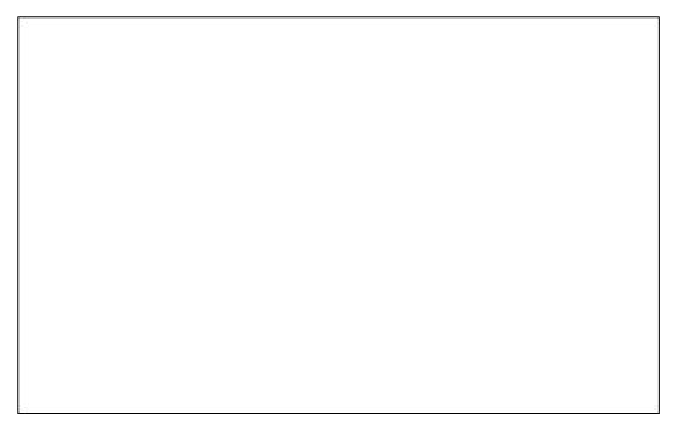
\includegraphics[width=0.45\textwidth]{High_view_of_CUDA_GPU_microarchitecture.eps}
\caption{ High View of CUDA CPU Microarchitecture
The GeForce GTX 760 has 6 SMs and the maximum number of threads allowed on each SM is 2048. Thus the total number of threads that can work in parallel is $2048\times 6=12288$.
}
\label{figure2}
\end{figure}   
% Note that IEEE does not put floats in the very first column - or typically
% anywhere on the first page for that matter. Also, in-text middle ("here")
% positioning is not used. Most IEEE journals/conferences use top floats
% exclusively. Note that, LaTeX2e, unlike IEEE journals/conferences, places
% footnotes above bottom floats. This can be corrected via the \fnbelowfloat
% command of the stfloats package.
\section{GPU Based Acceleration of FCSD}\label{GPUFCSD}
\subsection{MIMO System Model}\label{system}
% no \IEEEPARstart
%This demo file is intended to serve as a ``starter file''
%for IEEE conference papers produced under \LaTeX\ using
%IEEEtran.cls version 1.8 and later.
% You must have at least 2 lines in the paragraph with the drop letter
% (should never be an issue)
%I wish you the best of success.
%\hfill mds
%\hfill December 27, 2012

We consider a complex uncoded spatial multiplexing MIMO system with $N_r$ receive and $N_t$ transmit antennas, $N_{r}\geq N_{t}$, over a flat fading channel. Using a discrete time model, $\mathbf{y}\in\mathbb{C}^{N_{r}\times 1}$ is the received symbol vector written as:
\begin{equation}
\mathbf{y}=\mathbf{H}\mathbf{s}+\mathbf{n},   \label{formula 1}
\end{equation}
where $\mathbf{s}\in \mathbb{C}^{N_{t}\times 1}$ is the transmitted symbol vector, with components that are mutually independent and taken from a signal constellation $\mathbb{O}$ (4-QAM, 16-QAM, 64-QAM) of size $M$. All the possible transmitted symbol vectors $\mathbf{s}\in \mathbb{O}^{N_{t}}$, with $\mathbb{E}[\mathbf{s}\mathbf{s}^{H}]=\mathbf{I}_{N_t}E_{s}$, where $E_{s}$ denotes the symbol average energy, and $\mathbb{E}[\cdot]$ denotes the expectation operation. Furthermore $\mathbf{H}\in \mathbb{C}^{N_{r}\times N_{t}}$ denotes the Rayleigh fading channel propagation matrix with independent identity distributed (i.i.d) circularly symmetric complex Gaussian components of zero mean and unit variance. Finally, $\mathbf{n}\in \mathbb{C}^{N_{r}\times 1}$ is the additive white Gaussian noise (AWGN) vector with zero mean components and $\mathbb{E}[\mathbf{n}\mathbf{n}^{H}]=\mathbf{I}_{N_{r}}N_{0}$, where $N_{0}$ denotes the noise power spectrum density, and hence $\frac{E_{s}}{N_{0}}$ is the signal to noise ratio (SNR). 

Assume the receiver has the perfect channel state information (CSI), meaning that $ \mathbf{H}$ is known by receiver, as well as the SNR. The task of the MIMO decoder is to recover $\mathbf{s}$ based on $\mathbf{y}$ and $\mathbf{H}$.
\subsection{Fixed Complexity Sphere Decoder}
From (\ref{formula 1}), the maximum likelihood detector (MLD) for a MIMO system is specified by:
\begin{equation}
\mathbf{s}_{ML}=arg\min_{\mathbf{s}\in \mathbb{O}^{N_{t}}}||\mathbf{y}-\mathbf{H}\mathbf{s}||^{2}. \label{formula 2}
\end{equation}
We consider a MIMO system with  $N_{t}=N_{r}$. Performing the QR decomposition of the channel propagation matrix
\begin{equation}
 \mathbf{H}=\mathbf{Q}\mathbf{R},  \label{QR}
\end{equation}
where $\mathbf{Q}\in \mathbb{C}^{N_{t}\times N_{t}}$ is a unitary matrix and $\mathbf{R}\in \mathbb{C}^{N_{t}\times N_{t}}$, is an upper triangular matrix \cite{golub2012matrix}, we can write (\ref{formula 2}) as:
\begin{eqnarray}
\nonumber
\mathbf{s}_{ML}&=&arg\min_{\mathbf{s}\in \mathbb{O}^{N_{t}}}||\mathbf{Q}^{H}\mathbf{y}-\mathbf{Q}^{H}\mathbf{H}\mathbf{s}||^{2}\\
&=& arg\min_{\mathbf{s}\in \mathbb{O}^{N_{t}}}||\mathbf{Q}^{H}\mathbf{y}-\mathbf{R}\mathbf{s}||^{2}. \label{formula 3}
\end{eqnarray}
Using the unconstrained estimator of $\mathbf{s}$, $\mathbf{\hat{s}}=\mathbf{G}\mathbf{y}$, $\mathbf{G}=(\mathbf{H}^{H}\mathbf{H})^{-1}\mathbf{H}^{H}$, and (\ref{QR}), we have  
\begin{equation}
\mathbf{\hat{s}}=\mathbf{G}\mathbf{y}=(\mathbf{R}^{H}\mathbf{R})^{-1}\mathbf{R}^{H}\mathbf{Q}^{H}\mathbf{y}
=\mathbf{R}^{-1}\mathbf{Q}^{H}\mathbf{y}.
\label{unconstrained estimation}
\end{equation} 
Therefore $\mathbf{Q}^{H}\mathbf{y}=\mathbf{R}\mathbf{\hat{s}}$, and (\ref{formula 3}) can be written as
\begin{equation}
\mathbf{s}_{ML}=arg\min_{\mathbf{s}\in \mathbb{O}^{N_{t}}}||\mathbf{R}(\mathbf{\hat{s}}-\mathbf{s})||^{2}. \label{formula 4}
\end{equation}

Similarly to SD the FCSD also performs depth first searching. At the first $\rho$ node levels\footnote{when $N_{r}=N_{t}$ the FCSD can achieve the same diversity as the MLD if $\rho\geq \sqrt{N_{t}}-1$ \cite{barbero2008fixing}} the FCSD searches all the possible signal symbols in constellation $\mathbb{O}^{N_{t}}$, a process called the Full Expansion (FE) stage. Let $\mathbf{s}^{F}$ denote FCSD symbol vector candidates. For the symbols $s^{F}_{N_{t}}, s^{F}_{N_{t}-1}\dots s^{F}_{N_{t}-\rho+1}$, the FCSD has $M$ branch expansions at each symbol node. As shown in Fig. \ref{figure4}, there are $\rho=2$ FE node levels and each node level has $M=4$ branches. According to (\ref{formula 4}), we have: 
\begin{equation}
s^{F}_{i}=arg\min_{s\in \mathbb{O}^{N_{t}}}\{\sum_{i=1}^{N_{t}}|r_{ii}(\hat{s}_{i}-s^{F}_{i})+\sum_{j=i+1}^{N_{t}}r_{ij}(\hat{s}_{j}-s^{F}_{j})|^{2}\},  \label{formula 5}
\end{equation} 
$i\in [1,2\dots N_{t}]$, where $r_{ij}$ denotes the component at the $i$th row and $j$th column of the upper triangular matrix $\mathbf{R}$. Based on (\ref{formula 5}) at the remaining $N_{t}-\rho$ levels of symbols, the FCSD employs decision feedback, and therefore there are only one branch expansion for each symbol node at this stage. This stage is called Single Expansion (SE). 
Thus the total number of the branches is fixed, and the FCSD works as a constant number of multiple path tree searching algorithm.

In conclusion the FCSD symbol vector candidate $s^{F}_{i}=[s_{1},s_{2}\dots s_{N_{t}}]$ can be expressed as:
\begin{equation}
\begin{split}
&FE \quad stage:\\
&{s}_{i}^{F}\in    \mathbb{O}^{\rho},  \quad if\quad i=N_{t},N_{t}-1,\dots N_{t}-\rho+1\\
& SE\quad stage:\\
&{s}_{i}^{F}=\mathbb{Q}[\hat{s}_{i}+\sum_{j=i+1}^{N_{t}}\frac{r_{ij}}{r_{ii}}(\hat{s}_{j}-s_{j}^{F})], \quad if\quad \\
& i = N_{t}-\rho,N_{t}-\rho-1,\dots 2,1 
  \label{FCSD solution}
\end{split}
\end{equation}
where $\mathbb{Q}[\cdot]$ denotes the operation of signal constellation quantization. At the post processing stage, the FCSD compares the Euclidean distance of all the symbol vector candidates
\begin{equation}
E_{metric}=||\mathbf{R}(\mathbf{\hat{s}}-\mathbf{s}^{F})||^{2},
\end{equation} 
where $\mathbf{s}^{F}$ denotes the symbol vector candidate. The symbol vector candidate with minimum $E_{metric}$ is chosen as the solution. The total number of candidates is $M^{\rho}$.  
\begin{figure}[htb]
\centering
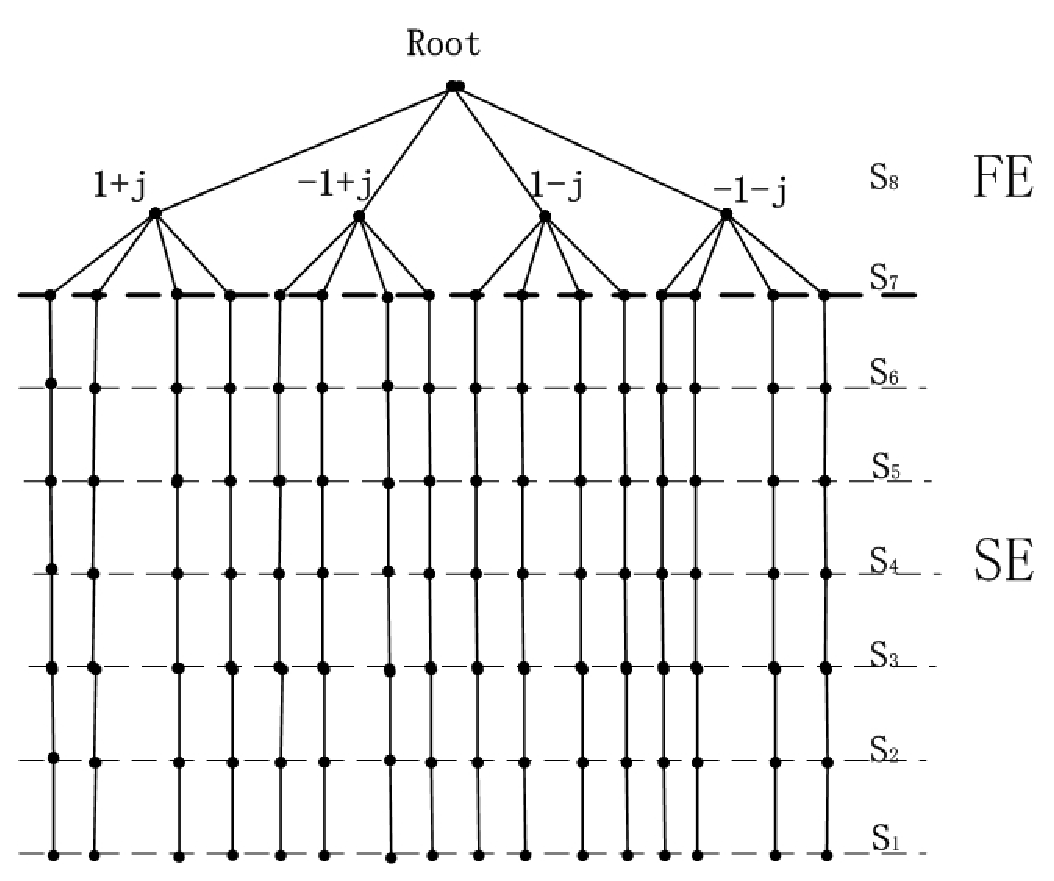
\includegraphics[width=0.5\textwidth, height=8cm]{FCSD_tree_searching.eps}
\caption{Tree searching of 4-QAM FCSD for 8$\times$8 MIMO system. The total number of branches is $4^{2}$}
\label{figure4}
\end{figure}
\subsection{CUDA-FCSD Preprocessing}
A FCSD channel ordering strategy is used in order to avoid error propagation in the serial path searching process. This channel ordering strategy is based on post processing signal to noise ratio\cite{wolniansky1998v}
\begin{equation}
\varphi_{m}=\frac{E_{s}}{\sigma^{2}(\mathbf{H}^{H}\mathbf{H})_{mm}^{-1}},  \label{ppsnr}
\end{equation}
where $\varphi_{m}$ denotes the post processing signal to noise ratio of the $m$th data stream, and $(\mathbf{H}^{H}\mathbf{H})_{mm}^{-1}$ denotes the diagonal elements of the inverse of $\mathbf{H}^{H}\mathbf{H}$. The post processing SNR depends only on $(\mathbf{H}^{H}\mathbf{H})_{mm}^{-1}$. From \cite{barbero2008fixing}, at the FE stage the "weakest" data stream, that is the data stream with the smallest $\varphi_{m}$, is detected first. At the SE stage, because of the single searching branch of the node, the performance is tightly related to the post processing SNR. Therefore at the SE stage the data stream with the largest post processing SNR is detected first in order to avoiding error propagation. In conclusion the FCSD ordering works iteratively  and obeys the following rule:
at the $j$th step ($j=1,2\dots N_{t}-1$), $s_{p}$ denotes the symbol to be detected, where 
\begin{equation}
p=\left\lbrace \begin{array}{c}
arg\max_{k}(\mathbf{H}_{j}^{H}\mathbf{H}_{j})_{kk}^{-1}\quad FE\quad stage\\
arg\min_{k}(\mathbf{H}_{j}^{H}\mathbf{H}_{j})_{kk}^{-1}\quad SE\quad stage   \label{the ordering}
\end{array}\right.  
\end{equation}  
and $\mathbf{H}_{j}\in \mathbb{C}^{N_{r}\times (N_{t}-j+1)}$ denotes the renewed channel matrix with the column corresponding to previous detected data streams removed from $\mathbf{H}_{j-1}$.

As mentioned in section \ref{programming model}, our implementation is based on the heterogeneous programming principle, employing a mix of CPU and GPU technology. The flow control and logical operations reside at the host side, while the compute intensive work is implemented at the device side. Although the FCSD preprocessing has a serial nature and can not be vectorized, the computational intensive operations can be performed by the CUDA Basic Linear Algebra Subprograms (cuBLAS)\cite{nvidia2013basic} and corresponding GPU program implementations, as shown in Table \ref{table1}.
\begin{table*}[htb]
\centering
\caption{Parallel Computation Operation of FCSD Preprocessing}
\begin{tabular}{|c|p{3cm}|p{3cm}|p{3cm}|p{3cm}|}
\hline
Operations & complex matrix-matrix multiplication & complex matrix-vector multiplication & matrix inverse & Cholesky factorization \\
\hline
GPU subroutine & $\mathit{cublasCgemm}$  & $\mathit{cublasCgemv}$ & $\mathit{GJE}$ & $\mathit{chol}$\\
\hline
Formula   &  $\mathbf{H}^{H}\mathbf{H}$ & $(\mathbf{H}^{H}\mathbf{H})^{-1}\mathbf{H}^{H}y$ & $(\mathbf{H}_{j}^{H}\mathbf{H}_{j})^{-1} $ & $\mathbf{H}^{H}\mathbf{H}=\mathbf{R}^{H}\mathbf{R}$ 
\\
\hline
\end{tabular}
\label{table1}
\end{table*}

\subsection{Parallel Acceleration of Paths Searching}
Since the decision feedback searching paths have a serial nature, we match one path to one thread. In order to have the largest number of threads that can be parallelized, we use one dimensional blocks for widest expansion, and organize all the paths into several such blocks. For example for a $16\times 16$ MIMO system with $16$QAM, the number of paths we need to search is $M^{\rho}=16^{3}=4096$, since $\rho=\lceil \sqrt{N_{t}}-1\rceil$, where $\lceil x\rceil$ represent the smallest integer greater than or equal to $x$. For largest SM occupancy we use 4 blocks for the path searching kernel where each block has 1024 threads which is the maximum number allowed per block. At each FCSD searching path, the following operations are performed in one thread:
\begin{itemize}
\item \emph{Path searching}\\
As in (\ref{FCSD solution}).
\item \emph{Euclidean Distance Calculation}
\begin{equation}
E_{u}^{k}=\sum_{i=1}^{i=N_{t}}\sum_{j=i}^{j=N_{t}}r_{ij}(\hat{s}_{j}-s^{F}_{j}), \label{Eu metric}
\end{equation}
\end{itemize}
where $E_{u}^{k}$ denotes the Euclidean distance of the $k$th symbol vector candidate. We integrate the post processing (\ref{Eu metric}) into the path searching process (\ref{FCSD solution}) to reduce the iteration times per thread.
 
In order to avoid low speed host-device data transfer, we reduce data transfers as much as possible. As shown in Fig. \ref{block diagram} we perform data transfer only two times. For host to device, the propagation channel matrix $\mathbf{H}$, received symbol vector $\mathbf{y}$, as well as the sub symbol vector index list $\mathit{s_{index}}$ at FE stage, are transferred. For device to host, the FCSD symbol vector solution $\mathbf{s}^{F}$ is transferred.
\begin{figure}[htb]
\centering
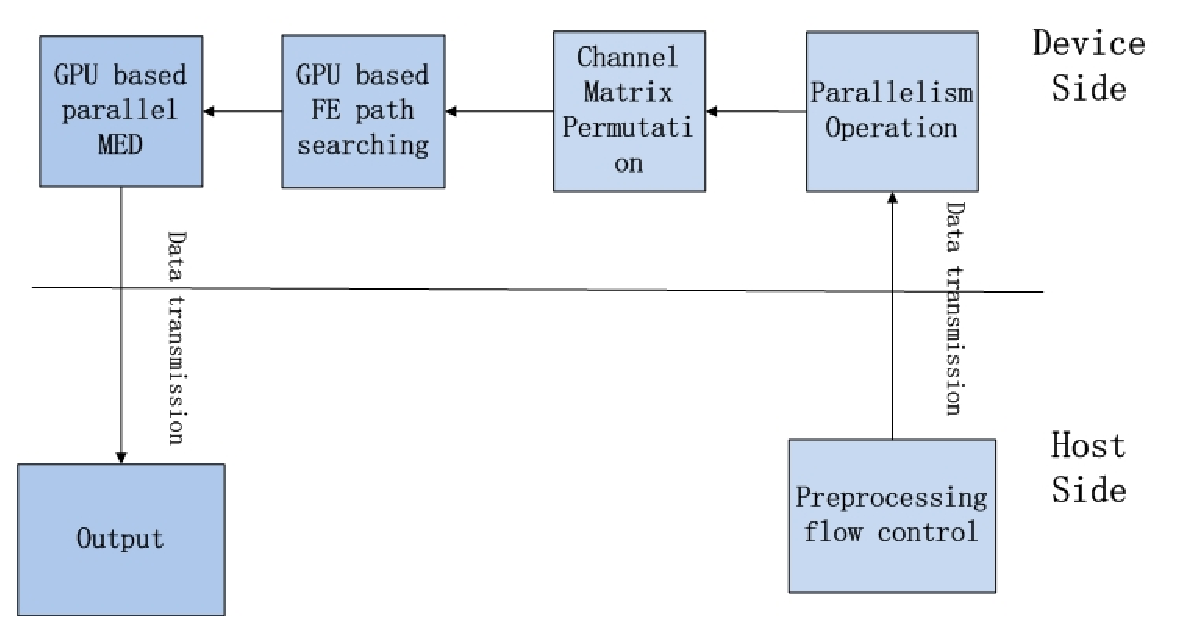
\includegraphics[width=0.5\textwidth, height=5.1cm]{CUDA_FCSD_block_diagram.eps}
\caption{Block Diagram of CUDA-FCSD Implementation}
\label{block diagram}
\end{figure}
\subsubsection{Data Preparation}\label{data preparation}
There are three major factors that influence the configuration of the data sets in memory space.
\begin{itemize}
\item Number of Reading Writing (R/W) operations
\item Valid program scope
\item Storage occupancy
\end{itemize}

Unlike CPUs that have a flat memory model (the CPU core can access any memory location by a near clock rate speed) GPUs are computation intensive. Thus the memory R/W operations are time consuming that influence performance. Furthermore different memory types have different program scopes. Local memory, which is invoked in \textit{kernel} functions is valid only in one thread. Shared memory is valid in one block. Constant, texture and global memories are valid both at host side and device side. On the other hand different from global memory, the constant and share memory are all capacity limited. Thus the memory occupancy is an important factor that needs to be considered.
 
At the host side we set four data sets that are stored in global memory. The $M^{\rho}\times N_{t}$ complex matrix $\mathit{s_{pm}}$ that stores in each row one symbol vector candidate and its program scope should be during the whole \textit{kernel} execution. The matrix $\mathit{s_{index}}$ is used to store the index of all the possible sub-symbol vectors for  FE stage using the full factorial method and requires a $\rho\times M^{\rho}$  integer matrix space. The $M^{\rho}$ dimensional floating point vector is used to store the Euclidean distance of all the symbol vector candidates. The $N_{t}$ dimensional complex vector $\mathit{s_{kernel}}$ is used to store the FCSD solutions and has to be transferred to host side.

On the other hand, the upper triangular matrix $\mathbf{R}$ and the unconstrained estimator $\mathbf{\hat{s}}$ of (\ref{unconstrained estimation}) are read only and require large numbers of read operations. Since these two data sets need small sizes of storage, the constant memory, which is cached and read only, is used to store them.
\subsubsection{Memory Accesss Pattern}
When considering a large MIMO system, the large number of required R/W operations make the memory bandwidth a major bottleneck for performance. Although the off-chip memory theoretical bandwidth is extremely high (the theoretical bandwidth of GeForce GTX 760 is 192GB/s), in practice it can only be achieved by a proper R/W strategy.

Global memory access is implemented by a dynamic random access memory (DRAM) whose R/W is an extremely slow process. In a modern DRAM the R/W operations are performed by accessing a piece of consecutive memory location. As mentioned in section \ref{programming model}, the warp is the basic schedule unit of a device, and memory space is accessed warp by warp. Thus the most effective global memory access pattern is to ensure a warp of threads can access a consecutive memory space. For the GeForce GTX 760, the DRAM will access a consecutive memory space of 128 bytes at one time. In Fig. \ref{coalesce global memory} we present the global access pattern of $\mathit{s_{pm}}$ as an example to illustrate global memory access pattern.
\begin{figure}[htb]
\centering
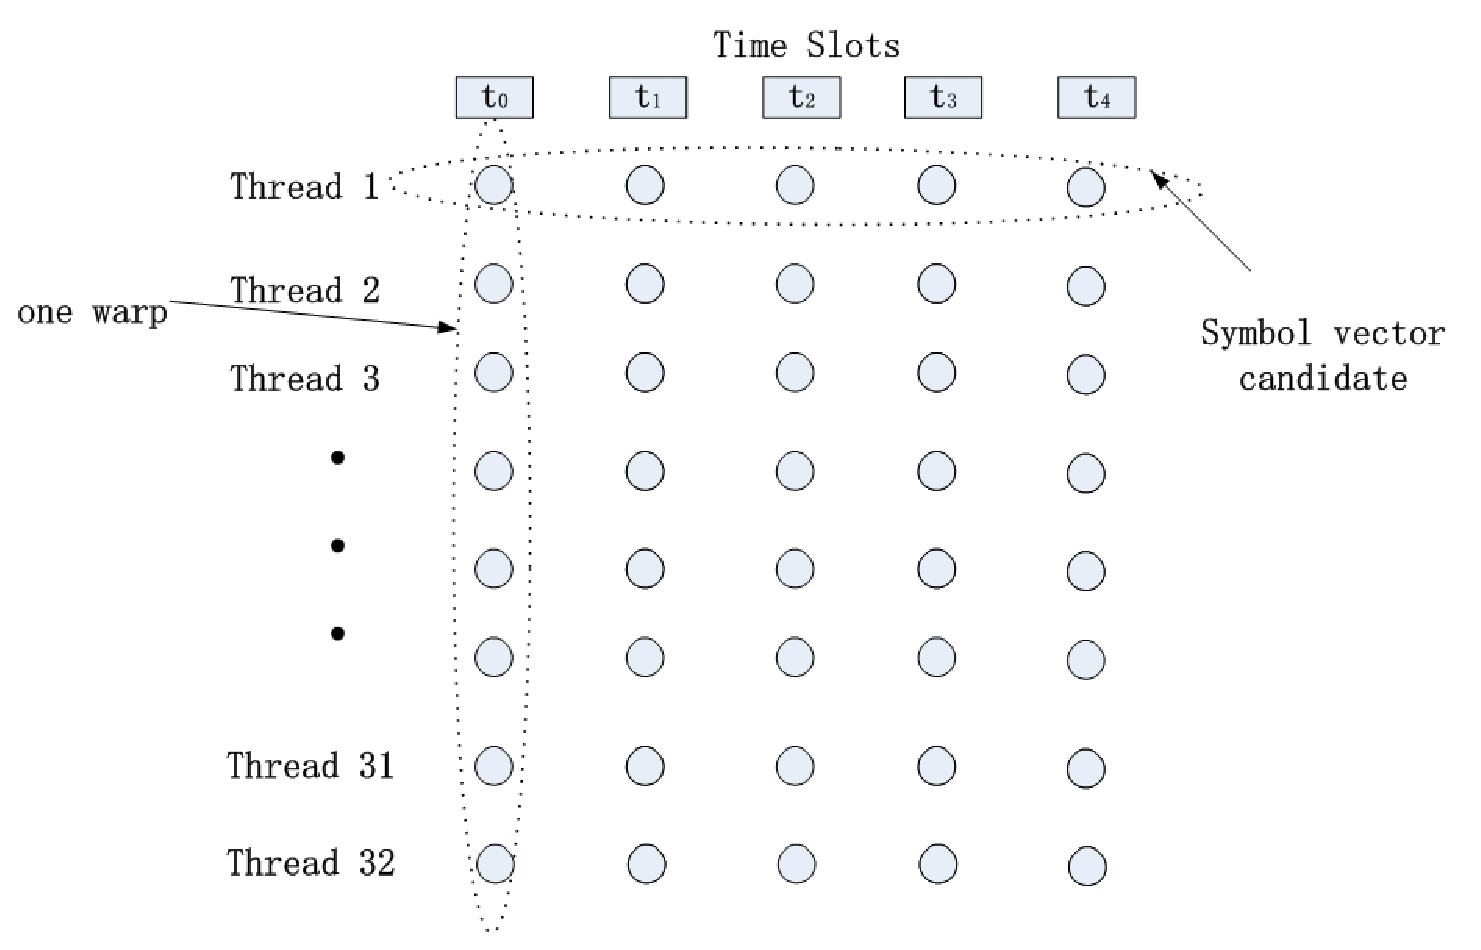
\includegraphics[width=0.5\textwidth, height=8cm]{coalescing_global_memory.eps}
\caption{Global Memory Access Pattern of $\mathit{s_{pm}}$}
\label{coalesce global memory}
\end{figure}


The complex matrix $\mathit{s_{pm}}$ is stored in one piece of linear global memory, where each row represents one $N_{t}$ complex symbols solution candidates of $\mathbf{\hat{s}}^{F}$ in (\ref{formula 5}). There are $M^{\rho}$ rows, and this matrix is stored in column major (first column in the first piece of memory space and the second in the second piece of memory space etc.). As mentioned before, one path searching is performed by one thread, and therefore the address distance between two consecutive symbols in one thread is $M^{\rho}$. However for consecutive threads in one warp, the address they reach is continuous as shown in Fig. \ref{coalesce global memory}. Every 32 threads in one warp can confirm R/W operations to a piece of memory that is consecutive, and reduce DRAM access as much as possible resulting in a better memory bandwidth.

All the thread level temporary data that is used in (\ref{FCSD solution}), (\ref{Eu metric}), and the symbol vector candidate during the path searching process, are stored in registers to get near clock rate access speed.   

\subsection{Larger MIMO Systems and Constellation Sizes}
There are two problems that need to be considered for large MIMO systems and constellation size:
\begin{itemize}
\item Thread resource limitation:
The number of threads that can be executed in parallel is limited. When the size of a MIMO system and constellation increases, it becomes impossible to parallelize all the searching paths in one \textit{kernel} execution. For example, in a $32\times 32$ MIMO system with $16$QAM modulation, the number of paths that need to be searched is $M^{\rho}=16^{5}=1048576$.  
\item Global memory limitation:
Large MIMO systems and large signal constellations require a large global memory space to store the symbol vector candidates. For example, for the systems $36\times 36$ with $16$QAM, $144\times 144$ with $4$QAM, $20\times 20$ with $64$QAM, the required space of storing $s_{pm}$ of section \ref{data preparation} exceeds the limit (2 GB).
\end{itemize}

One solution to these problems is to employ partial parallelism. The detection task is divided into several \textit{kernel} executions, where for each, only one potential symbol vector solution, as well as its corresponding Euclidean distance are preserved. This allows the global memory space to be reused to avoid exceeding its limit. 
\section{Simulation Results}\label{simulation}
\subsection{Environment}
\subsubsection{Device}
\begin{itemize}
\item \emph{Graphic Processing Units}: GeForce GTX 760, GPU clock rate: 1.08 GHz , memory clock rate 3 GHz , number of SM 6, maximum number of threads per stream multiprocessor 2048, total amount of global memory 2 GB, total amount of share memory per block 49 KB, total amount of constant memory 66 KB. 
\item \emph{Central Processing Units-Modigliani}: Intel Core I5-4th generation, 4 physical cores, 3.20 GHz CPU clock rate, 8 GB RAM.
\item \emph{Central Processing Units-Monet} : Intel Core I7-3rd generation, 6 physical cores, 3.20 GHz CPU clock rate, 32 GB RAM.
\end{itemize}
\subsubsection{Software}
\begin{itemize}
\item CUDA Driver Version / Runtime Version      6.5 / 6.0
\item Integrated software environment for source code editing, automatic building and debugging: Nsight Eclipse Version 6.5
\end{itemize}
\subsection{Performance Evaluation}
\begin{table*}[htb]
\centering
\caption{ Speedup Performance of Different MIMO Systems using 4 QAM}
\begin{tabular}{|c|c|c|c|c|c|}
\hline
\multirow{2}{*}{ Array size} & \multicolumn{3}{|c|}{Time/s} & \multicolumn{2}{|c|}{Speedup}\\
\cline{2-6}
&GeForce GTX 760 & Modigliani & Monet &  $\vartheta_{GTX 760}/\vartheta_{Modigliani}$  & $\vartheta_{GTX 760}/\vartheta_{Monet}$ \\
\hline
$8\times 8$& 7.39& 0.10&0.11 & 0.01& 0.01\\
\hline
$16\times 16$&16.26 & 0.92&0.98& 0.06& 0.06\\
\hline
$32\times 32$&38.32 & 31.27& 34.60& 0.82& 0.90\\
\hline
$48\times 48$&71.95& 262.00& 285.14& 3.64& 3.96\\
\hline
$64\times 64$& 322.90&1753.30&1940.10&5.43& 6.01 \\
\hline
$72\times 72 $&1285.41&8727.69 &9641.80 &6.79 &7.50 \\
\hline
$84\times 84$ &6454.02&47095.33&49962.01&7.30&7.74\\
\hline
\end{tabular}
\label{speedup1}
\end{table*}
\begin{table*}[htb]
\centering
\caption{ Speedup Performance of Different MIMO Systems using 16 QAM}
\begin{tabular}{|c|c|c|c|c|c|}
\hline
\multirow{2}{*}{ Array size} & \multicolumn{3}{|c|}{Time/s} & \multicolumn{2}{|c|}{Speedup}\\
\cline{2-6}
&GeForce GTX 760 & Modigliani & Monet &  $\vartheta_{GTX 760}/\vartheta_{Modigliani}$  &  $\vartheta_{GTX 760}/\vartheta_{Monet}$ \\
\hline
$8\times 8$&13.20& 0.67&0.93 & 0.05&0.07\\
\hline
$16\times 16$&26.80 & 31.68&41.95& 1.18& 1.57\\
\hline
$20\times 20$&192.70 & 740.50& 978.26& 3.84& 5.08\\
\hline
$32\times 32$&4980.13& 28209.53& 38106.00& 5.66& 7.65\\
\hline
$36\times 36$& 5568.26&35240.16&47290.00&6.33& 8.61 \\
\hline
\end{tabular}
\label{speedup2}
\end{table*}
\begin{table*}[htb]
\centering
\caption{Speedup Performance of Different MIMO Systems using 64 QAM}
\begin{tabular}{|c|c|c|c|c|c|}
\hline
\multirow{2}{*}{ Array size} & \multicolumn{3}{|c|}{Time/s} & \multicolumn{2}{|c|}{Speedup}\\
\cline{2-6}
&GeForce GTX 760 & Modigliani & Monet &  $\vartheta_{GTX 760}/\vartheta_{Modigliani}$  &  $\vartheta_{GTX 760}/\vartheta_{Monet}$ \\
\hline
$8\times 8$&12.28& 10.69&13.38 & 0.87&1.09 \\
\hline
$16\times 16$&468.92 & 2066.08&2689.00& 4.41& 5.73\\
\hline
\end{tabular}
\label{speedup3}
\end{table*}
Monte-Carlo simulations were conducted for MIMO systems of different sizes and signal constellation. In this work the speedup is defined as $\vartheta_{GPU}/\vartheta_{CPU}$, where $\vartheta_{GPU}$ and $\vartheta_{CPU}$ denotes the number of symbols detected on GPU and CPU per second. Comparison is made between the GeForce GTX 760 and two types of CPUs, with speedup performance presented in Tables \ref{speedup1}, \ref{speedup2} and \ref{speedup3}. All the operation times correspond to $1000$ channel realizations.

From Table \ref{speedup1}, we see that for small MIMO systems of $8\times 8$, $16\times 16$, and $32\times 32$ with $4$QAM, the speed performance of GPU implementation is worse than that of CPU. The number of paths of these MIMO configurations that need to be searched is relatively small\footnote{$8\times 8$ MIMO system with $4$QAM has $16$ paths, $16\times 16$ MIMO system with $4$QAM has $64$ paths and $32\times 32$ MIMO system with $4$QAM has $1024$ paths}. The CPUs are designed for serial code execution with special hardware (branch prediction units, multiple caches, etc.) that provide extremely good performance, while the GPUs can achieve good performance only when they are utilized in a massive parallel manner. Furthermore there is a short time for GPU to "warm up", for host-device data transmission, \textit{kernel} function  launching and host device synchronization. When comes to larger MIMO systems of $48\times 48$, $64\times 64$, $72\times 72$, a large parallelism is achieved allowing the GPU to begin displaying its data processing power. 

In Tables \ref{speedup2} and \ref{speedup3}, $16$QAM and $64$QAM are considered. We see that speedups larger than 1 can be achieved with GPU implementation also with smaller MIMO systems. For a $16\times 16$ system with $16$QAM modulation, GTX 760 provides a $1.18$ speedup over Modigliani and $1.57$ speedup over Monet. For a $16\times 16$ system with $64$QAM, GTX 760 provides a $4.41$ speedup over Modigliani and $5.73$ speedup over Monet. The nature of FCSD is such that for lager signal constellations, massive parallelism can be reached also for small MIMO systems that are not extremely large.

It can be observed from Tables \ref{speedup1}, \ref{speedup2} and \ref{speedup3}, that the GPU implementation shows its speed advantage over CPU implementation for increasing size of MIMO systems and signal constellations, indicating that GPUs provide advantages for large MIMO system with large signal constellations.

In Fig. \ref{BER curve} we present Monte Carlo simulation results for bit error rate (BER) performance, using the GPU implementation of different MIMO system configurations and constellation sizes. We consider uncoded complex MIMO systems with $M$QAM, where each antenna transmits different streams of binary data generated randomly and independently. The results have been obtained by using $100000$ channel realizations with at least $500$ symbol errors accumulated. The simulation results show that FCSD-CUDA provides the same BER performance as its CPU version\cite{barbero2008fixing}.
\begin{figure}[htb]
\centering
\includegraphics*[width=0.56\textwidth]{BER_curves.eps}
\caption{BER performance for MIMO systems with various modulation schemes using the GPU implementation}
\label{BER curve}
\end{figure}
\section{Conclusions}\label{conclusion}
This paper presents a GPU implementation of the fixed complexity sphere decoder (FCSD) for large MIMO systems. In order to exploit the computational capability of GPU in the simulation of large MIMO systems, the utilization of a heterogeneous programming model, accounting for resource limitations and memory configuration must be considered. The simulation results show that a considerable acceleration of the GPU implementation of FCSD can be reached for large MIMO systems and signal constellation sizes over CPU implementation, while maintaining the same BER performance. Since the GPU and CPU can work independently, the data processing power of GPU computing is an additional advantages provided by the traditional simulation platforms. This shows the potential of GPU computing to reduce the time associated with intensive simulations of large MIMO systems.


% conference papers do not normally have an appendix


% use section* for acknowledgement
%\section*{Acknowledgment}








% trigger a \newpage just before the given reference
% number - used to balance the columns on the last page
% adjust value as needed - may need to be readjusted if
% the document is modified later
%\IEEEtriggeratref{8}
% The "triggered" command can be changed if desired:
%\IEEEtriggercmd{\enlargethispage{-5in}}

% references section

% can use a bibliography generated by BibTeX as a .bbl file
% BibTeX documentation can be easily obtained at:
% http://www.ctan.org/tex-archive/biblio/bibtex/contrib/doc/
% The IEEEtran BibTeX style support page is at:
% http://www.michaelshell.org/tex/ieeetran/bibtex/
%\bibliographystyle{IEEEtran}
% argument is your BibTeX string definitions and bibliography database(s)
%\bibliography{IEEEabrv,../bib/paper}
%
% <OR> manually copy in the resultant .bbl file
% set second argument of \begin to the number of references
% (used to reserve space for the reference number labels box)






% that's all folks
%\end{spacing}
\bibliographystyle{IEEEtran}
\bibliography{IEEEabrv,citationconf}
\end{document}